\section{Results} \label{sec_res}
In this section, we show two Fourier analyses of MIP: one where the $S_n$ order is
varied and one where the aspect ratio is varied. We also compare different
methods to solve MIP: congugate gradient (CG), conjugate gradient
preconditioned with symmetric Gauss-Seidel (PCG-SGS), conjugate gradient
preconditioned with ML using uncoupled aggregation (PCG-MLU),
conjugate gradient preconditioned with ML using MIS aggregation (PCG-MLM),
and AGMG. The options used for ML can be found in the Appendix.
\subsection{Fourier Analyses}
Analysing Source Iteration accelerated with DSA is often performed using
Fourier analysis \cite{larsen_dsa,consistent_p1}. When a Fourier analysis is
performed, the error is decomposed into different modes and by inspecting the 
damping of the different error modes, the effectiveness of the DSA scheme can 
be studied. The largest damping factor is the spectral radius of the method. 
The smaller the spectral radius is, the faster the scheme converges. If the 
spectral radius is greater than one, the method is unstable. 
\subsubsection{$S_n$ order varied}
This Fourier analysis was carried on a square cell, using a
Gauss-Legendre-Chebyshev (GLC) quadrature. The medium is homogeneous, the scattering
ratio $c=0.9999$ and periodic boundary conditions are used. The $x-$axis is the mesh
size in mean free path and the $y-$axis is the spectral radius. On Figure
\ref{fig_fa_op}, there are four curves corresponding to different $S_n$ order: 
$S_2$, $S_4$, $S_8$, and $S_{16}$.
\begin{figure}[H]
  \centering
  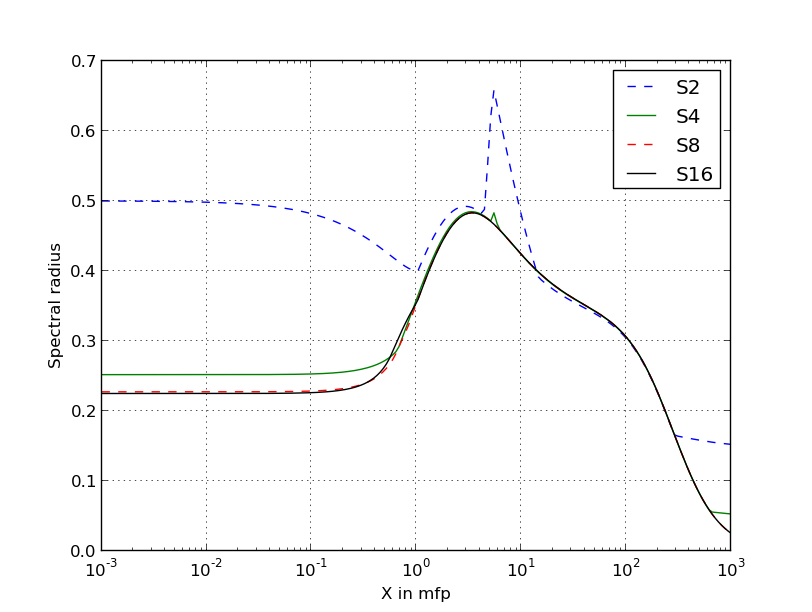
\includegraphics[width=0.5\textwidth]{./Dsa/sn_order_9999}
  \caption{Fourier analysis as a function of the mesh optical thickness,
  homogeneous infinite medium case.}
  \label{fig_fa_op}
\end{figure}
MIP is stable for every cell size. The spectral radius is always less than
0.5, except for $S_2$ where it peaks at about 0.7.
\subsubsection{Aspect ratio varied}
For this Fourier analysis, we use a $S_{16}$ GLC quadrature, a homogeneous
medium, $c=0.9999$ and periodic boundary conditions. The $x-$axis is the mesh
size in mean free path in the $x$ direction and the $y-$axis is the spectral
radius. On Figure \ref{fig_fa_ar}, there are five curves corresponding to five 
different aspect ratio: $\frac{Y}{X}=\frac{1}{16}$, $\frac{Y}{X}=\frac{1}{4}$, 
$\frac{Y}{X}=1$, $\frac{Y}{X}=4$, $\frac{Y}{X}=16$, and $\frac{Y}{X}=100$. 
\begin{figure}[H]
  \centering
  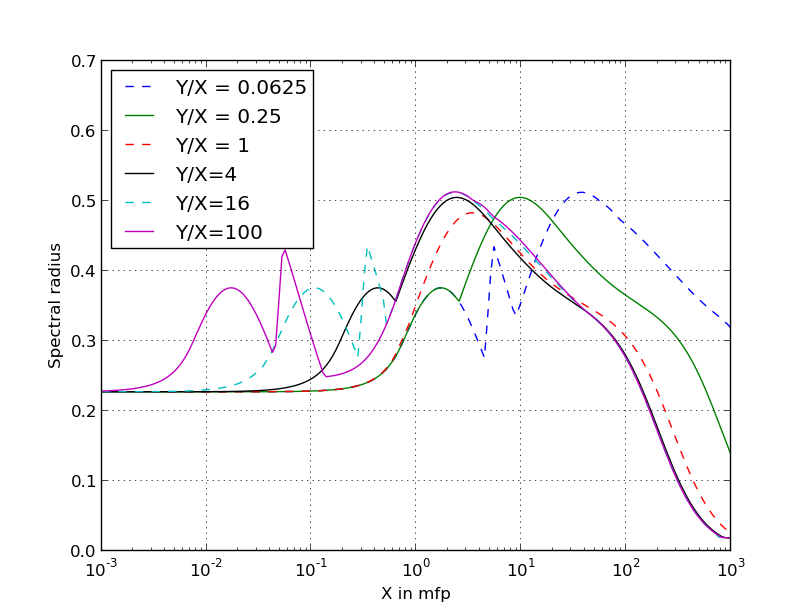
\includegraphics[width=0.5\textwidth]{./Dsa/aspect_ratio_9999_2}
  \caption{Fourier analysis as a function of the mesh optical thickness,
  homogeneous infinite medium case for different aspect ratios.}
  \label{fig_fa_ar}
\end{figure}
MIP is stable for every aspect ratio and the maximum of the spectral radius
peaks at about 0.5

\subsection{Homogeneous medium}
Next, we compare different solvers for MIP on a homogeneous medium, 10cm $\times$
10cm, $\Sigma_t=1$cm$^{-1}$ and $\Sigma_s=0.999$cm$^{-1}$, with vacuum boundary 
conditions and a source of intensity 1cm$^{-3}$s$^{-1}$. We use a $S_8$
Gauss-Legendre-Chebyshev quadrature, a Source Iteration solver with relative
tolerance of $10^{-8}$ and a relative tolerance for MIP of $10^{-10}$.
\begin{description}
  \item[Quadrilateral cells:] the mesh is composed of 49236 quadrilateral cells
    that corresponds to 197052 degrees of freedom.
  \item[Polygonal cells:] the mesh is composed of 45204 triangles, 823 
    quadrilaterals, 4978 pentagons, 4155 hexagons, 725 heptagons, and 24 
    octagons, for a total of 55909 cells and 193991 degrees of freedoms. This 
    example will allow us to test MIP and the different preconditioners on a 
    mesh composed of different types of cell.
\end{description}
The meshes and the solutions of these two problems are given on Figure
\ref{fig_meshes_phi}:
\begin{figure}[H]
\centering    
\subfloat[Quadrilateral cells]{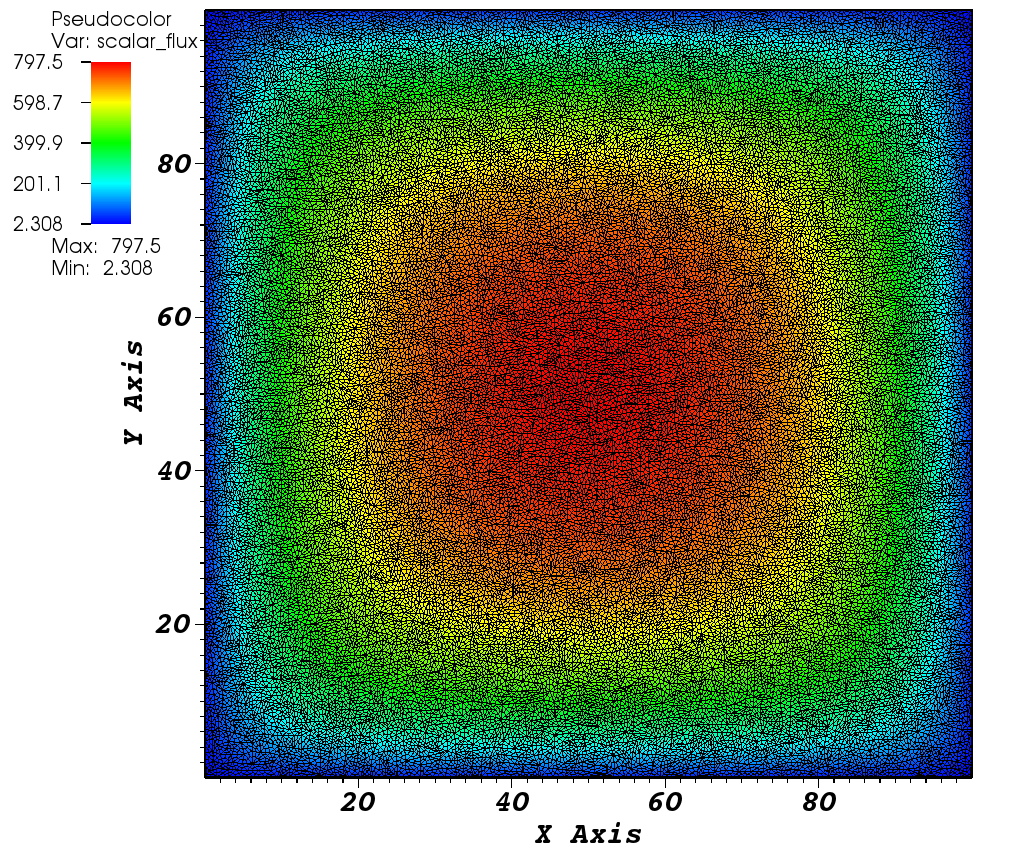
\includegraphics[width=0.45\textwidth]
  {./Dsa/big_homog_quad_crop}}
\subfloat[Polygonal cells]{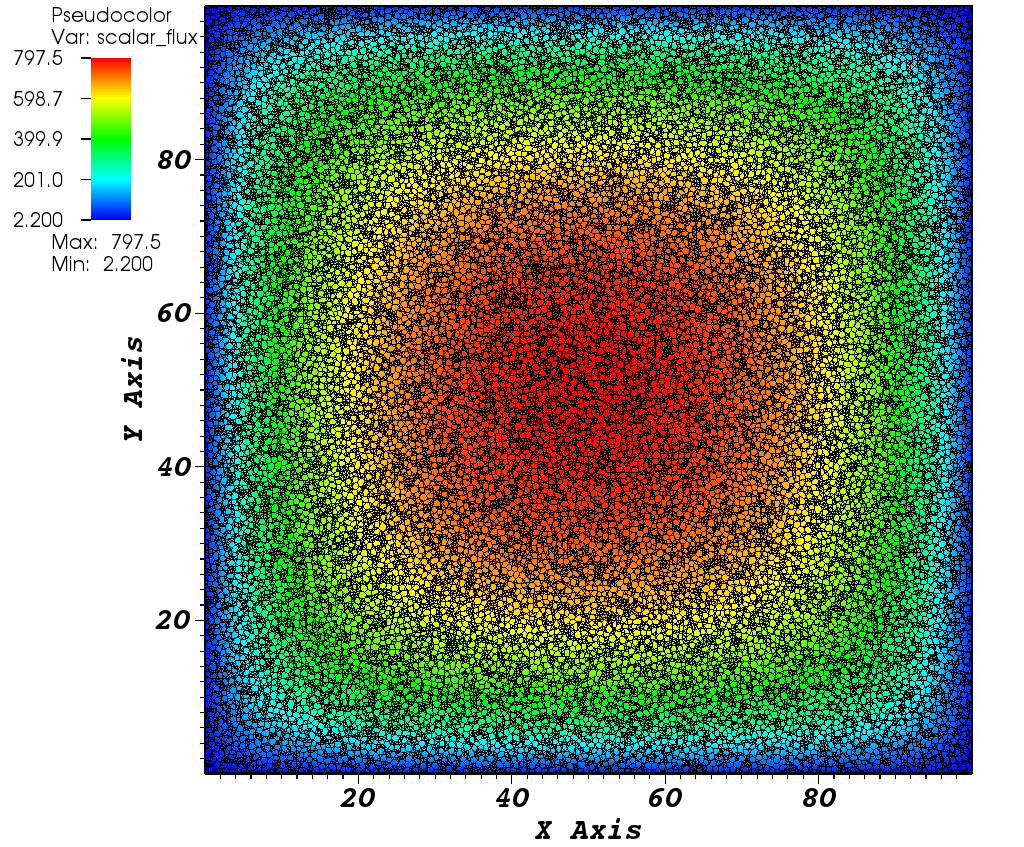
\includegraphics[width=0.45\textwidth]
  {./Dsa/big_homog_poly_crop}}
\caption{Meshes and scalar fluxes}
\label{fig_meshes_phi}
\end{figure}

In the next table, the different solvers, used on the quadrilateral cells, 
are compared:
\begin{table}[H]
\begin{center}
\caption{Comparison of different preconditioners for quadrilateral cells.}
\begin{tabular}{|c|c|c|c|c|c|c|}
\hline
& No-DSA & CG & PCG-SGS &  PCG-MLU & PCG-MLM & AGMG\\
\hline
SI iter   & 7311    & 24      & 24       & 24      & 24      & 24      \\
Prec (s)  & NA      & NA      & 0.171358 & 1.8255  & 9.56078 & 0.332   \\
MIP (s)   & NA      & 1095.7  & 1311.76  & 192.622 & 197.632 & 29.9727 \\
CG iter   & NA      & 56649   & 17332    & 630     & 604     & 578     \\
Total (s) & 39176.7 & 1264.98 & 1477.95  & 363.202 & 367.841 & 194.568 \\
\hline
\end{tabular}
\end{center}
\end{table}
In this Table, SI iter is the number iteration of Source Iteration
needed to solve the problem, Prec is the time in seconds needed to
initialize the preconditioner used by CG, MIP is the total time in
seconds spent solving DSA during the calculation, CG iter is the total number 
of CG iterations used to solve MIP, and Total is the time in
seconds needed to solve the problem.

Using MIP decreases significantly the number of SI iterations and the
calculation time as expected. Using PCG-SGS decreases by a 
factor three the number of CG iterations compared to CG but the time 
needed to solve MIP is greater. With ML, the number of CG iterations is 
reduced by a factor 50 and the MIP calculation time is divided by three 
compared to CG. AGMG is by far the most efficient solver, the number of 
CG iteration is slightly lower than PCG-ML but the MIP calculation is 20 
times faster than CG.

The different solvers, used on the polygonal cells, are compared in the next Table:
\begin{table}[H]
\begin{center}
\caption{Comparison of different preconditioners for polygonal cells.}
\begin{tabular}{|c|c|c|c|c|c|c|}
\hline
& No-DSA & CG & PCG-SGS & PCG-MLU & PCG-MLM & AGMG\\
\hline
SI iter   & 7311    & 23      & 23      & 23      & 23      & 23      \\
Prec (s)  & NA      & NA      & 0.06388 & 1.73379 & 8.0426  & 0.388   \\
MIP (s)   & NA      & 877.861 & 1263.31 & 198.63  & 191.989 & 31.242  \\
CG iter   & NA      & 46262   & 16712   & 652     & 603     & 555     \\
Total (s) & 42666.7 & 1060.53 & 1447.53 & 382.275 & 384.422 & 216.946 \\
\hline
\end{tabular}
\end{center}
\end{table}
We see that using different types of cells in the same mesh does not affect
the performance of MIP or of the preconditioners. 

\subsection{Heterogeneous medium}
In this example, we use a heterogeneous medium composed of 184 triangles, 3720
quadrilaterals and 2791 regular hexagons of side 0.05$cm$ for a total of 6695 
cells and 32178 degrees of freedom. The domain is 5.28275$cm$ by 4.6$cm$. 
Reflective boundary conditions are used. The quadrature is a $S_{16}$ 
Gauss-Legendre-Chebyshev quadrature. The SI solver has a relative tolerance of 
$10^{-8}$ and the relative tolerance for MIP is $10^{-10}$. The domain is 
composed of three zones (see Figure \ref{fig_zone_hex}:
\begin{figure}[H]
  \centering
  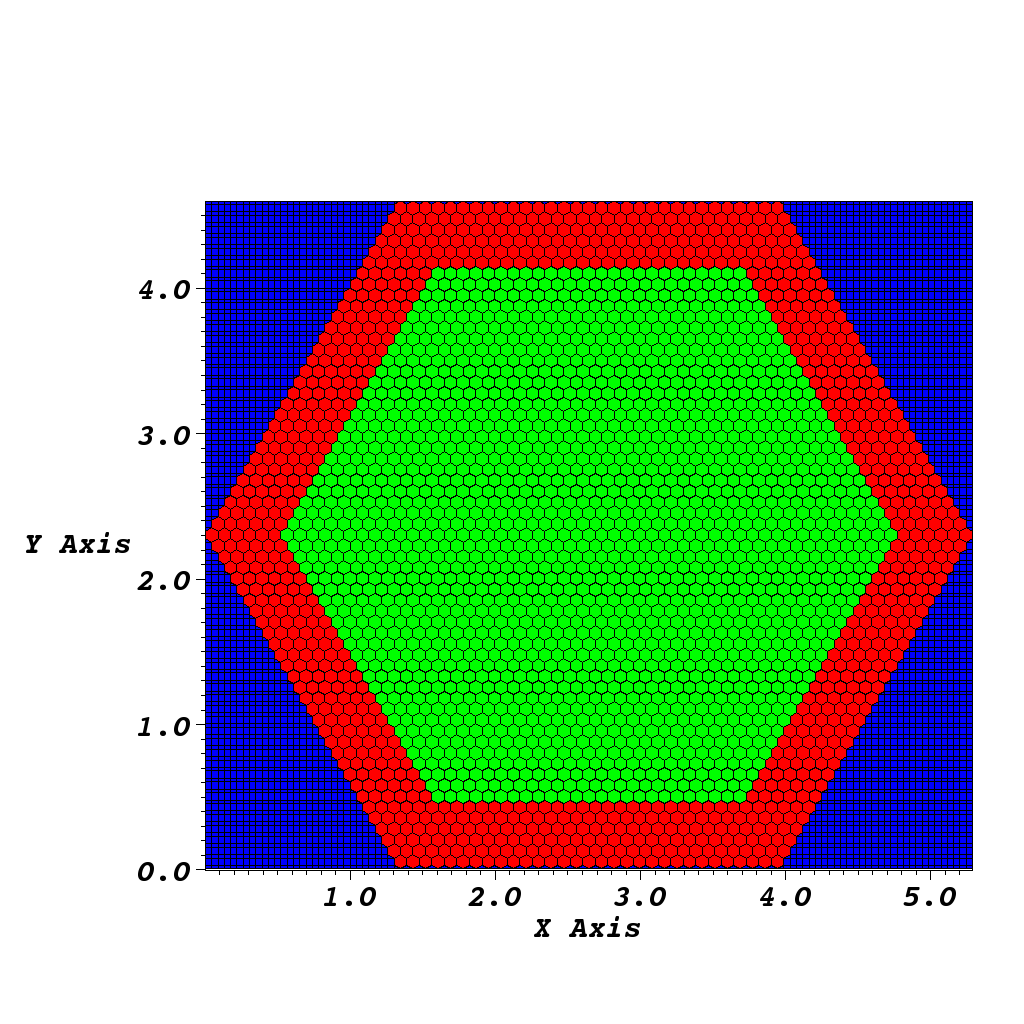
\includegraphics[width=0.4\textwidth]{./Dsa/source_crop}
  \caption{Zones of the domain.}
  \label{fig_zone_hex}
\end{figure}
The properties of the different zones are:
\begin{description}
  \item[Green zone:] $\Sigma_t =1.5$cm$^{-1}$, $\Sigma_s = 1.44$cm$^{-1}$, source$ =
    1$cm$^{-3}$s$^{-1}$
  \item[Red zone:] $\Sigma_t = 1$cm$^{-1}$, $\Sigma_s = 0.9$cm$^{-1}$, no source
  \item[Blue zone:] $\Sigma_t = 1$cm$^{-1}$, $\Sigma_s = 0.3$cm$^{-1}$, no source
\end{description}
The different solvers are compared in the next Table:
\begin{table}[H]
  \begin{center}
    \caption{Comparison of different preconditioners for a heterogeneous medium.}
    \begin{tabular}{|c|c|c|c|c|c|c|}
      \hline
      & No-DSA & CG & PCG-SGS & PCG-MLU & PCG-MLM & AGMG\\
      \hline
      SI iter   & 122      & 18      & 18       & 18       & 18      & 18 \\
      Prec (s)  & NA       & NA      & 0.016149 & 0.336215 & 1.36803 & 0.065 \\
      MIP (s)   & NA       & 60.2031 & 123.05   & 31.7048  & 30.8669 & 2.80108\\
      CG iter   & NA       & 12016   & 6764     & 423      & 391     & 248 \\
      Total (s) & 413.274  & 131.297 & 188.586  & 101.888  & 103.734 & 71.5392\\
      \hline
    \end{tabular}
    \caption{Comparison of preconditioners with heterogeneous medium.}
  \end{center}
\end{table}
We can see that the comments that were done for the homogeneous tests are
still valid. MIP is effective even with heterogeneous medium and AGMG is
still the fastest solver.

The cross sections of the different zones were taken from \cite{mip}. In the
next test, they are modified to make the problem more challenging:
\begin{description}
  \item[Green zone:] $\Sigma_t =1.5$cm$^{-1}$, $\Sigma_s = 1.499$cm$^{-1}$, source$ =
    1$cm$^{-3}$s$^{-1}$
  \item[Red zone:] $\Sigma_t = 1$cm$^{-1}$, $\Sigma_s = 0.999$cm$^{-1}$, no source
  \item[Blue zone:] $\Sigma_t = 1$cm$^{-1}$, $\Sigma_s = 0.3$cm$^{-1}$, no source
\end{description}
The different solvers are compared in the next Table:
\begin{table}[H]
  \begin{center}
    \caption{Comparison of different preconditioners for a heterogeneous medium.}
    \begin{tabular}{|c|c|c|c|c|c|c|}
      \hline
      & No-DSA & CG & PCG-SGS & PCG-MLU & PCG-MLM & AGMG\\
      \hline
      SI iter   & 278     & 17      & 17        & 17       & 17      & 17 \\
      Prec (s)  & NA      & NA      & 0.0160661 & 0.368768 & 1.41632 & 0.07 \\
      MIP (s)   & NA      & 58.422  & 126.93    & 33.2225  & 31.3045 & 2.924 \\
      CG iter   & NA      & 12214   & 6679      & 415      & 386     & 248 \\
      Total (s) & 910.566 & 120.889 & 190.413   & 99.7524  & 97.4666 & 70.6424 \\
      \hline
    \end{tabular}
    \caption{Comparison of preconditioners with heterogeneous medium.}
  \end{center}
\end{table}

\subsection{AMR mesh}
In this example from \cite{mip}, the domain is $10cm\times 10cm$. The left and bottom
boundaries are reflective whereas the right and the top boundaries are vacuum. 
There are 10720 cells: 10482 quadrilaterals, 236 pentagons,
and 2 hexagons for a total of 43120 degrees of freedom. 
As in the previous example, the domain is composed if three zones (see Figure
\ref{fig_zone_amr}:
\begin{figure}[H]
  \centering
  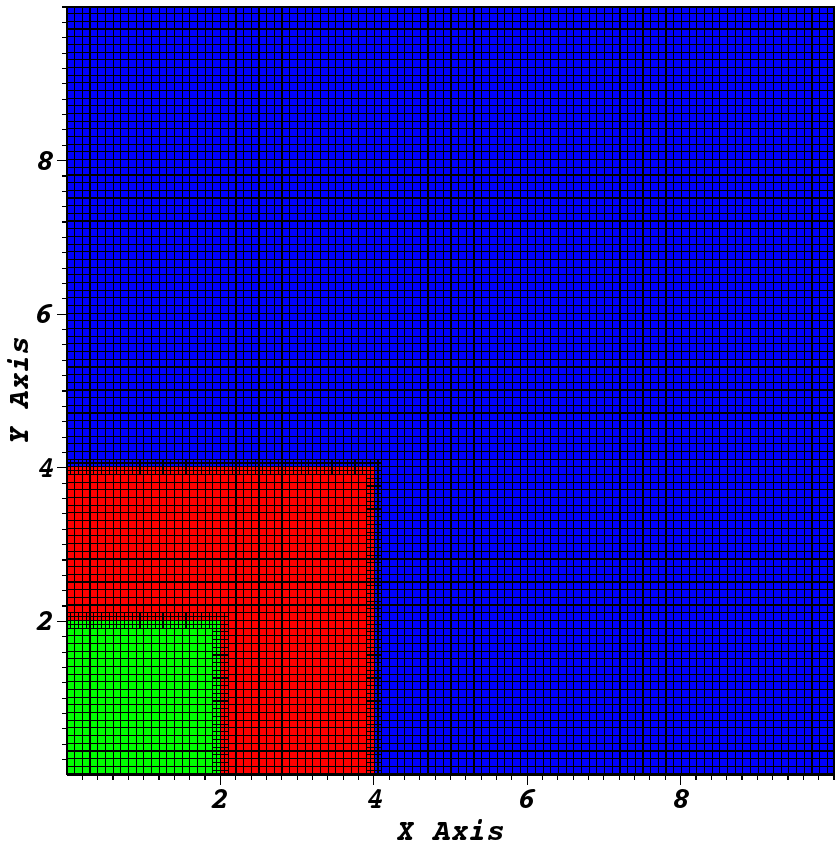
\includegraphics[width=6cm]{./Dsa/zone_amr}
  \caption{Polygons distribution}
  \label{fig_zone_amr}
\end{figure}
where:
\begin{description}
  \item[Green zone:] $\Sigma_t=1.5cm^{-1}$, $\Sigma_s=1.44cm^{-1}$,
    source=$1cm^{-3}s^{-1}$
  \item[Red zone:] $\Sigma_t=1cm^{-1}$, $\Sigma_s=0.9cm^{-1}$, no source
  \item[Blue zone:] $\Sigma_t=1cm^{-1}$, $\Sigma_s=0.3cm^{-1}$, no source
\end{description}
The distribution of cells is given on Figure \ref{fig_distr}:
\begin{figure}[H]
  \centering
  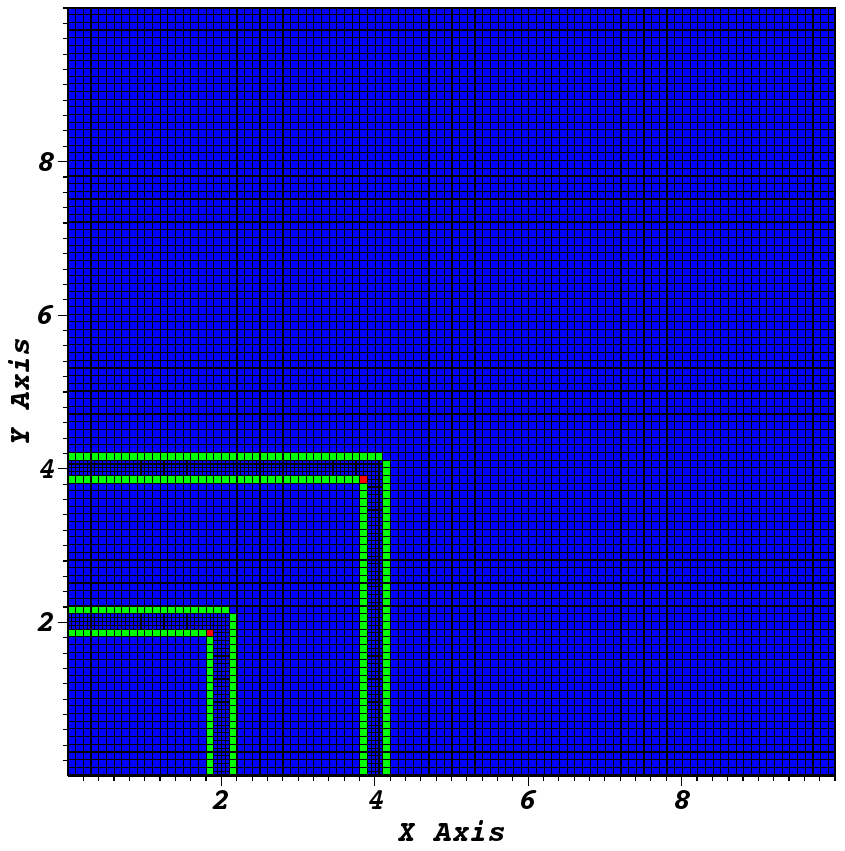
\includegraphics[width=6cm]{./Dsa/polygon_amr}
  \caption{Polygons distribution}
  \label{fig_distr}
\end{figure}
where:
\begin{description}
  \item[Blue cells] are quadrilaterals.
  \item[Green cells] are pentagons.
  \item[Red cells] are hexagons.
\end{description}
This mesh is typical of a mesh obtained after one level of adaptive mesh
refinement (the cells at the interface of different zones have been refined
once). We see that instead of introducing hanging nodes, we have introduce
pentagons and hexagons in the mesh.
A $S_{16}$ GLC quadrature is employed. The tolerance on SI is $10^{-8}$ and
the tolerance on the CG solvers is $10^{-10}$.
The different solvers are compared in the next Table:
\begin{table}[H]
  \caption{Comparison of preconditioners on AMR mesh.}
  \begin{center}
    \begin{tabular}{|c|c|c|c|c|c|c|}
      \hline
       & No-DSA & CG & PCG-SGS & PCG-MLU & PCG-MLM & AGMG \\
      \hline
      SI iter    & 184     & 19      & 19       & 19      & 19       & 19 \\
      Prec (s)   & NA      & NA      & 0.043463 & 0.358002 & 1.19301 & 0.0111\\
      MIP (s)    & NA      & 48.1908 & 81.0992  & 25.2699 & 25.0699  & 
      2.56198\\
      CG iter    & NA      & 11300   & 4734     & 361     & 361      & 264 \\
      Total (s)  & 802.985 & 138.825 & 172.423  & 116.018 & 116.517  &
      94.1963\\
      \hline
    \end{tabular}
  \end{center}
\end{table}
As expected, the results are similar to our previous tests.

\subsection{Rectangular cells}
\emph{\red{I have to redo this example to have at least one example of MIP
with BLD.}}\\
Like mentioned previously in this Chapter, AMG can have difficulties when the
aspect ratio of rectangular cells is high. Moreover, when the aspect ratio is high,
MIP becomes ill conditioned. In the next example, the domain is 
square $3cm \times 3cm$ with vacuum boundaries, 300 divisions along x-axis, 
and 30 divisions along y-axis. There 9000 cells and since PWLD finite elements, 
there are 36000 degrees of freedom. The relative tolerance on SI is $10^{-8}$ 
and the relative tolerance on CG is $10^{-10}$. We use a $S_{8}$ GLC quadrature, 
$\Sigma_t = 1 cm^{-1}$, and $\Sigma_s = 0.999 cm^{-1}$.

In this example, the aspect ratio $Y/X = 10$. We
also compared the effect of the size of the coarsest grid on the convergence.
In the next Table, we compare No-DSA, CG, and AGMG defined previously with:
\begin{description}
  \item[PCG-MLU-D:] conjugate gradient preconditioned with ML
    using uncoupled coarsening with a coarsest grid of size less 
    or equal of 128 (default value).
  \item[PCG-MLU-M:] conjugate gradient preconditioned with ML
    using uncoupled coarsening with a coarsest grid of size less 
    or equal of 400 (same value than AGMG).
  \item[PCG-MLM-D:] conjugate gradient preconditioned with ML
    using MIS coarsening with a coarsest grid of size less or 
    equal of 128 (default value).
  \item[PCG-MLM-M:] conjugate gradient preconditioned with ML
    using MIS coarsening with a coarsest grid of size less or 
    equal of 400 (same value than AGMG).
\end{description}
\begin{landscape}
  \begin{center}
    \begin{table}[H]
      \caption{Comparison of preconditioners on rectangular mesh.}
      \begin{centering}
        \begin{tabular}{|c|c|c|c|c|c|c|c|c|}
          \hline
          & No-DSA & CG & PCG-SGS & PCG-MLU-D & PCG-MLU-M & PCG-MLM-D &
          PCG-MLM-M & AGMG \\
          \hline
          SI iter    & 62      & 26      & 26       & 26       & 26       & 
            26       & 26       &  26 \\
          Prec (s)   & NA      & NA      & 0.015177 & 0.300424 & 0.310577 &
            0.900931 & 0.847251 & 0.044 \\
          MIP (s)    & NA      & 115.936 & 249.85   & 157.941  & 153.097  & 
            154.04   & 147.658  & 6.22109\\
          CG iter    & NA      & 29623   & 16675    & 2674     & 2674     & 
            2619     & 2619     & 810 \\
          Total (s)  & 62.6123 & 146.177 & 249.15   & 188.184  & 182.458  & 
            185.008  & 177.297  & 33.1472\\
          \hline
        \end{tabular}
      \end{centering}
    \end{table}
  \end{center}
\end{landscape}
We can see that at the exception of AGMG, all the other preconditioned 
conjugate gradients performed significantly worse than for the others test 
cases. AGMG does not seem to be affected by the ill conditioning of MIP or the 
high aspect ratio. The change of coarsest grid size does not have a significant 
effect on the time needed to solve MIP.
